\section{Plano de integração e validação} % (fold)
\label{sec:plano_de_integração_e_validação}
	Após implementar os subsistemas é necessário planjear a maneira como será realizada a integração entre eles, as figuras \ref{img:integração_robô} e \ref{img:integração_base} apresentam de maneira geral as relações existentes entre os subsistemas de acordo com as implmementações realizadas.

	\begin{figure}[H]                                                           
   		\centering                                                                
   		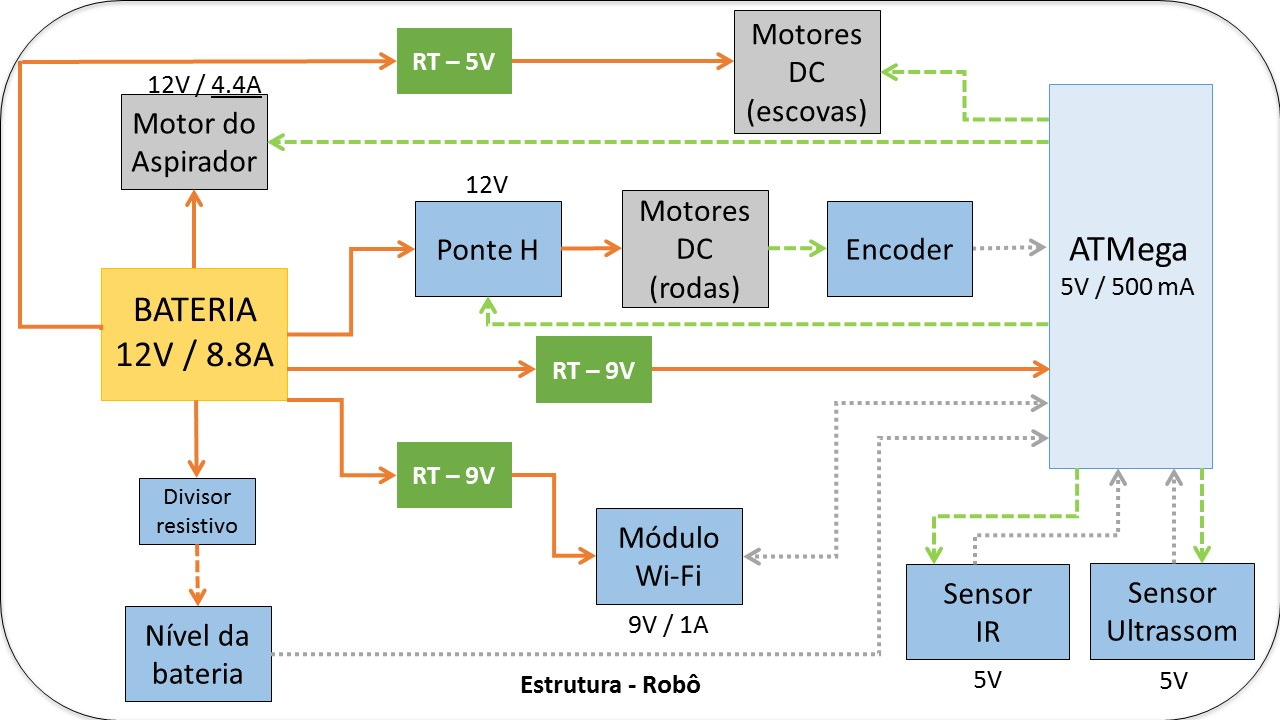
\includegraphics[scale=0.5]{figuras/plano_integracao_robo.jpg}               
   		\caption{Plano geral de integração dos subsistemas par ao robô.}    
   		\label{img:integração_robô}                                            
   	\end{figure} 

   	\begin{figure}[H]                                                           
   		\centering                                                                
   		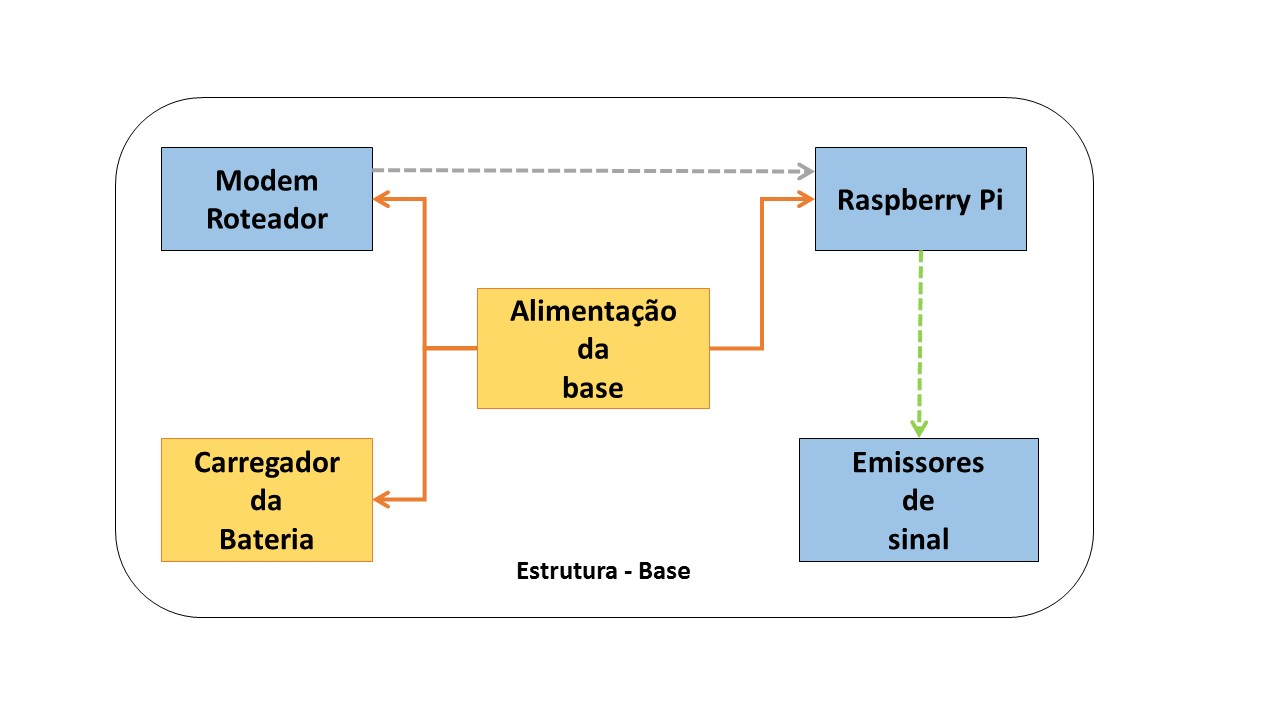
\includegraphics[scale=0.5]{figuras/plano_integracao_base.jpg}               
   		\caption{Plano geral de integração dos subsistemas para a base.}    
   		\label{img:integração_base}                                            
   	\end{figure} 

   	\noindent \textbf{Legenda}: \\
   	\noindent \textit{Setas de cor verde} - simbolizam que determinado bloco tem controle sobre um outro bloco. \\
   	\noindent \textit{Setas de cor laranja} - simbolizam a allimentação necessária para os componentes. \\
   	\noindent \textit{Setas de cor cinza} - simbolizam que há comunicação entre os blocos (os sentidos das setas indicam os caminhos dos dados).
% section plano_de_integração_e_validação (end)